\documentclass[table]{beamer}
\usepackage[utf8]{inputenc}
\usepackage[brazilian]{babel}
\usepackage{amsmath}
\usepackage{graphicx}
\usepackage{hyperref}
\usepackage{ragged2e}   
\usepackage{epstopdf}
\usepackage{multirow}
\usepackage{minted}
\usepackage{booktabs}

\setbeamertemplate{sidebar right}{}
\setbeamertemplate{footline}{%
\hfill\usebeamertemplate***{navigation symbols}
\hspace{1cm}\insertframenumber{}/\inserttotalframenumber}

\addtobeamertemplate{block begin}{}{\justifying}  %new code

\setbeamertemplate{footline}
{
  \leavevmode%
  \hbox{%
  \begin{beamercolorbox}[wd=.333333\paperwidth,ht=2.25ex,dp=1ex,center]{author in head/foot}%
    \usebeamerfont{author in head/foot}\insertsection
  \end{beamercolorbox}%
  \begin{beamercolorbox}[wd=.333333\paperwidth,ht=2.25ex,dp=1ex,center]{title in head/foot}%
    \usebeamerfont{title in head/foot}\insertsubsection
  \end{beamercolorbox}%
  \begin{beamercolorbox}[wd=.333333\paperwidth,ht=2.25ex,dp=1ex,right]{date in head/foot}%
    \usebeamerfont{date in head/foot}\insertshortdate{}\hspace*{2em}
    \insertframenumber{} / \inserttotalframenumber\hspace*{2ex} 
  \end{beamercolorbox}}%
  \vskip0pt%
}

\begin{document}

\begin{frame}
   \frametitle{Compiladores}
   \large
   \begin{center}
   Análise Semântica
   \end{center}
   \scriptsize
   \begin{center}
      João Marcelo Uchôa de Alencar \\
      joao.marcelo@ufc.br \\
      UFC-Quixadá
   \end{center}
\end{frame}

\begin{frame}
   \tableofcontents
\end{frame}

\section{Introdução}
\begin{frame}
   \frametitle{Análise Semântica}
   \begin{itemize}
      \item Estrutura sintática do programa já conhecida;
      \item computar informações além da capacidade das gramáticas livres de contexto;
      \item análise semântica \textbf{estática}: 
      \begin{itemize}
         \item Ocorre antes da execução;
         \item tabela de símbolos para acompanhar o significado de nomes;
	 \item inferência e verificação de tipos.
      \end{itemize}
      \item análise pelas regras da linguagem, para verificar correção e garantir execução;
      \item análise efetuada pelo compilador para melhorar eficiência;
      \item não há como determinar a correção completa do programa.
   \end{itemize}
\end{frame}

\begin{frame}
   \frametitle{Análise Semântica}
   \begin{itemize}
      \item Não existe um método padrão como a BNF para especificar a semântica estática;
      \item \textbf{atributos}:
      \begin{itemize}
         \item equações de atributos ou regras semânticas;
	 \item gramática de atributos;
	 \item semântica dirigida pela sintaxe.
      \end{itemize}
      \item O desenvolvedor de compiladores deve construir uma gramática de atributos manualmente;
      \item sintaxe abstrata;
      \item múltiplas passadas:
      \begin{itemize}
         \item Analisador semântico concorrente ao sintático é complexo;
	 \item a prática moderna indica o uso de múltiplas passadas.
      \end{itemize}
      \item não há um \textbf{gerador de analisador semântico} consolidado como \textit{lex} e \textit{yacc}.
   \end{itemize}
\end{frame}

\section{Atributos e Gramáticas de Atributos}
\begin{frame}
   \frametitle{Atributos e Gramáticas de Atributos}
   \begin{block}{Atributos}
   Qualquer propriedade de uma construção de linguagem de programação.
   \begin{itemize}
      \item Tipo de dados de uma variável;
      \item valor de uma expressão;
      \item localização de uma variável na memória;
      \item código objeto de um procedimento;
      \item quantidade de dígitos significativos em um número.
   \end{itemize}
   \end{block}
   O processo de computar um atributo e associar seu valor computado com a construção da linguagem é chamado de \textbf{amarração} (ligação ou \textit{binding}). \\
   O momento durante a compilação ou execução em que ocorre a amarração é o \textbf{tempo de amarração} (tempo de ligação ou \textit{binding time}).
\end{frame}

\begin{frame}
   \frametitle{Exemplos de Tempo de Ligação}
   \begin{block}{Tipos de dados}
   Durante a compilação, um \textbf{verificador de tipos} é um analisador semântico que computa o atributo de tipo de todas as entidades tipadas e verifica se os valores computados estão de acordo com as regras da linguagem.
   \end{block}
   \begin{block}{Valor de uma Expressão}
   Os valores de expressão em geral são dinâmicos, definidos em tempo de execução, mas o compilador precisa gerar código para calcular esses valores.
   \end{block}
\end{frame}

\begin{frame}
   \frametitle{Exemplos de Tempo de Ligação}
   \begin{block}{Localização de uma Variável na Memória}
   Pode ser definida durante a compilação ou execução, mas em geração é feita na geração de código, pois depende do sistema de memória alvo. 
   \end{block}
   \begin{block}{Código Objeto de um Procedimento}
   É atribuído durante a compilação, quando o procedimento também é compilado.
   \end{block}
   \begin{block}{Quantidade de Dígitos Significativos}
   A definição é feita fora do processo de compilação, pois considera detalhes da arquitetura. O compilador simplesmente aceita um valor definido pelo desenvolvedor do compilador.
   \end{block}
\end{frame}

\begin{frame}
   \frametitle{Gramáticas de Atributos}
   Na \textbf{semântica dirigida pela sintaxe}, os atributos são diretamente associados aos símbolos gramaticais da linguagem (os terminais e não terminais). Se $X$ for um símbolo gramatical, e $a$ um atributo, $X.a$ é o valor de $a$ associado a $X$. 
   \begin{block}{Equação Semântica}
   Seja uma regra $X_{0}\to X_{1}X_{2}...X_{n}$ e uma coleção de atributos $a_{1},...,a_{k}$: \\
   $X_{i}.a_{j}=f_{ij}(X_{0}.a_{1},...,X_{0}.a_{k},X_{1}.a_{1},...,X_{1}.a_{k},...,X_{n}.a_{1},...,X_{n}.a_{k})$
   \end{block}
   É \textbf{raro} que um atributo dependa de um número muito grande de outros atributos.
\end{frame}

\begin{frame}
   \frametitle{Gramáticas de Atributos}
   \begin{table}
      \begin{tabular}{cc}
      Regra Gramatical & Regras Semânticas \\
      \hline 
      Regra 1 & Equações de atributos associadas \\
        .     & . \\
        .     & . \\
        .     & . \\
      Regra $n$ & Equações de atributos associadas \\
      \hline
      \end{tabular}
   \end{table}
\end{frame}

\begin{frame}
   \frametitle{Gramáticas de Atributos - Exemplos}
   $\textit{número}\to\textit{número dígito}|\textit{dígito}$ \\
   \vspace{1.0cm}
   $\textit{dígito}\to0|1|2|3|4|5|6|7|8|9$ \\
   Considerado o atributo $val$ como representando o valor numérico a ser armazenado na memória, como seria a gramática de atributos?
\end{frame}

\begin{frame}
   \frametitle{Gramáticas de Atributos - Exemplos}
   \begin{table}
      \begin{tabular}{cc}
      Regra Gramatical & Regras Semânticas \\
      \hline 
       $\textit{número}\to\textit{número dígito}$ & $\textit{número}_{1}.val=$                          \\
                                                  & $\textit{número}_{2}.val*10 + \textit{dígito}.val$  \\
       $\textit{número}\to\textit{dígito}$        & $\textit{número}.val=\textit{dígito}.val$           \\
       $\textit{dígito}\to0$                      & $\textit{dígito}.val=0$                             \\
        .     & . \\
        .     & . \\
        .     & . \\
       $\textit{dígito}\to9$                      & $\textit{dígito}.val=9$                             \\
      \hline
      \end{tabular}
   \end{table}
   Como fica a árvore de análise sintática anotada com as computações de atributos para o número 345?
\end{frame}

\begin{frame}
   \frametitle{Gramáticas de Atributos - Exemplos}
   $exp\to exp+termo|exp-termo|termo$ \\
   $termo\to termo*fator|fator$ \\
   $fator\to (exp)|\textbf{número}$ \\
   Considerado o atributo $val$ como representando o valor numérico a ser atribuído a expressão, como seria a gramática de atributos?
\end{frame}

\begin{frame}
   \frametitle{Gramática de Atributos - Exemplos}
   \begin{table}
      \begin{tabular}{cc}
      Regra Gramatical & Regras Semânticas \\
      \hline 
      $exp_{1}\to exp_{2} + termo$ & $exp_{1}.val = exp_{2}.val + termo.val $ \\
      $exp_{1}\to exp_{2} - termo$ & $exp_{1}.val = exp_{2}.val - termo.val $ \\
      $exp\to termo$ & $exp.val = termo.val $ \\
      $termo_{1}\to termo_{2} * fator$ & $termo_{1}.val = termo_{2}.val - fator.val $ \\
      $termo\to fator$ & $termo.val = fator.val $ \\
      $fator\to (exp)$ & $fator.val = exp.val $ \\
      $fator\to \textbf{número}$ & $fator.val = \textbf{número.}val $ \\
      \hline
      \end{tabular}
   \end{table}
   Não existem equações com \textbf{número}.\textit{val} à esquerda. Como são calculados? \\
   Como ficaria a árvore de análise sintática para $(34-3)*42$.
\end{frame}

\begin{frame}
   \frametitle{Gramáticas de Atributos - Exemplos}
   $decl\to\textit{tipo var-lista}$ \\
   $tipo\to \textbf{int}|\textbf{float}$ \\
   $\textit{var-lista} \to \textbf{id},\textit{var-lista} | \textbf{id}$ \\
   Queremos definir um atributo \textit{dtipo} para identificadores e escrever equações para calculá-lo. 
\end{frame}

\begin{frame}
   \frametitle{Gramáticas de Atributos - Exemplos}
   \begin{table}
      \begin{tabular}{cc}
      Regra Gramatical & Regras Semânticas \\
      \hline 
      $decl\to \textit{tipo var-lista}$                              & $\textit{var-lista}.dtipo = tipo.dtipo$            \\
      $tipo\to \textbf{int}$                                         & $tipo.dtipo = integer$                             \\
      $tipo\to \textbf{float}$                                       & $tipo.dtipo = real$                                \\
      $\textit{var-lista}_{1}\to\textbf{id},\textit{var-lista}_{2}$  & $\textbf{id}.dtipo = \textit{var-lista}_{1}.dtipo$ \\
                                                                     & $\textit{var-lista}_{2}.dtipo = \textit{var-lista}_{1}.dtipo$ \\
      $\textit{var-lista}\to\textbf{id}$                             & $\textbf{id}.dtipo = \textit{var-lista}.dtipo$ \\
      \hline
      \end{tabular}
   \end{table}
   Como ficaria a árvore de análise sintática para a cadeia \textit{float x,y}?
\end{frame}

\begin{frame}
   \frametitle{Gramáticas de Atributos - Exemplos}
   $\textit{base-num}\to\textit{num basecar}$ \\
   $basecar\to\textbf{o}|\textbf{d}$ \\
   $num\to\textit{num dígito}|\textit{dígito}$ \\ 
   $\textit{dígito}\to0|1|2|3|4|5|6|7|8|9$ \\
   Como calcular o valor dos números nas duas bases diferentes? Será um único atributo suficiente?
\end{frame}

\begin{frame}
   \frametitle{Gramáticas de Atributos - Exemplos}
   \scriptsize
   \begin{table}
      \begin{tabular}{cc}
      Regra Gramatical & Regras Semânticas \\
      \hline 
      $\textit{base-num} \to \textit{num basecar}$ & $\textit{base-num}.val = num.val$ \\
                                                   & $num.base = basecar.base$         \\
      $basecar \to \textbf{o}$                     & $basecar.base = 8$                \\
      $basecar \to \textbf{d}$                     & $basecar.base = 10$               \\
      $num_{1} \to num_{2}\textit{dígito}$         & $num_{1}.val  =$                  \\
                                                   & $\textbf{if } \textit{dígito}.val = erro \textbf{ ou } \textit{num}_{2}.val = erro $  \\
                                                   & $\textbf{then } erro$ \\
                                                   & $\textbf{else } num_{2}.val*num_{1}.base+\textit{dígito}.val$ \\
                                                   & $num_{2}.base = num_{1}.base$ \\
                                                   & $\textit{dígito}.base = num_{1}.base$ \\
      $num \to \textit{dígito}$                    & $num.val = \textit{dígito}.val$ \\
                                                   & $\textit{dígito}.base = num_{1}.base$ \\
      $\textit{dígito}\to0$                        & $\textit{dígito}.val = 0$ \\
      . & . \\
      . & . \\
      . & . \\
      $\textit{dígito}\to8$                        & $\textit{dígito}.val =$ \\
                                                   & $\textbf{if } \textit{dígito}.base = 8 \textbf{ then } erro \textbf{ else } 8$ \\
      $\textit{dígito}\to9$                        & $\textit{dígito}.val =$ \\
                                                   & $\textbf{if } \textit{dígito}.base = 8 \textbf{ then } erro \textbf{ else } 9$ \\
 
      \hline
      \end{tabular}
   \end{table}
   Como ficaria a árvore de análise sintática para o número 345o?
\end{frame}

\begin{frame}[fragile]
   \frametitle{Simplificações das Gramáticas de Atributos}
   \begin{itemize}
      \item A coleção de expressões permitidas em uma equação de atributos é denominada \textbf{metalinguagem} para a gramática de atributos;
      \item \textbf{if-then-else, case, switch} serão utilizados, mas fica entendido que no projeto do compilador, a linguagem em que o mesmo é escrito será utilizada;
      \item também podemos usar funções que são definidas em outro lugar, por exemplo, uma função $\textit{dígito}.val = numval(D)$ poderia ser definida como:
      \begin{minted}{c}
      int numval(char D) {
        return (int)D - (int)'0'; 
      }
      \end{minted}
   \end{itemize}
\end{frame}

\begin{frame}
   \frametitle{Simplificações das Gramáticas de Atributos}
   Uma vez que a sintaxe já foi verificada, podemos simplificar a gramática: \\
   $exp\to exp + exp | exp - exp | exp * exp | (exp) | \textbf{número}$ \\
   \begin{table}
      \begin{tabular}{cc}
      Regra Gramatical & Regras Semânticas \\
      \hline 
      $exp_{1}\to exp_{2} + exp_{3}$ & $exp_{1}.val = exp_{2}.val + exp_{3}.val $ \\
      $exp_{1}\to exp_{2} - exp_{3}$ & $exp_{1}.val = exp_{2}.val - exp_{3}.val $ \\
      $exp_{1}\to exp_{2} * exp_{3}$ & $exp_{1}.val = exp_{2}.val * exp_{3}.val $ \\
      $exp_{1}\to (exp_{2})$         & $exp_{1}.val = exp_{2}.val $ \\
      $exp\to \textbf{número}$   & $exp.val = \textbf{número}.val $ \\
      \hline
      \end{tabular}
   \end{table}
   Como ficaria a \textbf{árvore de sintaxe abstrata} para $(34-3)*42$?
\end{frame}

\begin{frame}
   \frametitle{Simplificações das Gramáticas de Atributos}
   Podemos construir a árvore de sintaxe abstrata usando métodos auxiliares:
   \begin{itemize}
      \item \textit{mkOpNode}: recebe três parâmetros (marca do operador e duas árvores) e constrói um novo nó;
      \item \textit{mkNumNode}: recebe um parâmetro, valor numérico, e constrói um nó folha para esse valor.
   \end{itemize}
\end{frame}

\begin{frame}
   \frametitle{Simplificações das Gramáticas de Atributos}
   \begin{table}
      \begin{tabular}{cc}
      Regra Gramatical & Regras Semânticas \\
      \hline 
      $exp_{1}\to exp_{2} + termo$ & $exp_{1}.\textit{árvore} = $ \\
                                   & $mkOpNode(+,exp_{2}.\textit{árvore}, termo.\textit{árvore}) $ \\
      $exp_{1}\to exp_{2} - termo$ & $exp_{1}.\textit{árvore} = $ \\
                                   & $mkOpNode(-,exp_{2}.\textit{árvore}, termo.\textit{árvore}) $ \\

      $exp\to termo$ & $exp.\textit{árvore} = termo.\textit{árvore} $ \\
      $termo_{1}\to termo_{2} * fator$ & $termo_{1}.\textit{árvore} =$ \\
                                       & $mkOpNode(*, termo_{2}.\textit{árvore}, fator.\textit{árvore})$ \\
      $termo\to fator$ & $termo.\textit{árvore} = fator.\textit{árvore} $ \\
      $fator\to (exp)$ & $fator.\textit{árvore} = exp.\textit{árvore} $ \\
      $fator\to \textbf{número}$ & $fator.\textit{árvore} = $ \\
                                 & $mkNumNode(\textbf{número}.lexval)$ \\
      \hline
      \end{tabular}
   \end{table}
\end{frame}

\begin{frame}
   \frametitle{Algoritmos para Computação de Atributos}
   \begin{block}{O Problema}
   Encontrar uma ordem para a avaliação e atribuição de atributos que garanta que todos os outros atributos necessários já estejam disponíveis.
   \end{block}
   \begin{block}{Grafo de Dependências}
   Dado um atributo $X_{i}.a_{j}$ com $X_{i}$ em uma regra gramatical $X_{0}\to X_{1}X_{2}...X_{n}$, \textbf{existe um nó} para esse atributo no grafo de dependências. Considerando que: \\
   \begin{center}
   $X_{i}.a_{j} = f(...,X_{m}.a_{k},...)$ \\
   \end{center}
   é a equação de atributos associada, \textbf{existe uma aresta} de cada $X_{m}.a_{k}$ direcionada para o nó $X_{i}.a_{j}$.
   \end{block}
\end{frame}

\begin{frame}
   \frametitle{Construção do Grafo de Dependências}
   Considerando a gramática de atributos para números decimais, a regra $\textit{número}_{1}\to\textit{número}_{2}\textit{ dígito}$
tem a seguinte equação de atributos associada:
   \begin{center}
   $\textit{número}_{1}.val = \textit{número}_{2}.val * 10 + \textit{dígito}.val$
   \end{center}
   Considerando a regra de definição de nós e vértices, teremos:
   \begin{center}
   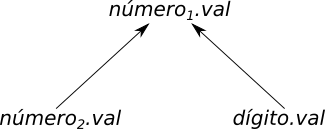
\includegraphics[scale=0.6]{figuras/exemplo66.png}
   \end{center}
   Para a cadeia 345, no próximo \textit{slide}, mostramos o grafo completo.
\end{frame}

\begin{frame}
   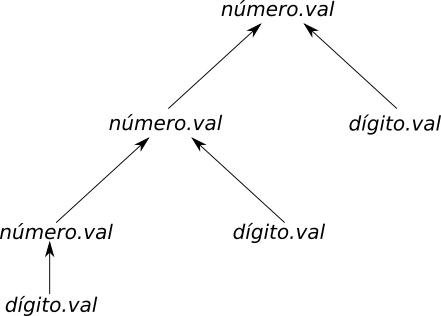
\includegraphics[width=\linewidth,height=\textheight,keepaspectratio]{figuras/exemplo66completo.png}
\end{frame}

\begin{frame}
   \frametitle{Construção do Grafo de Dependências}
   Para a regra gramatical:
   \begin{center}
   $\textit{var-lista}_{1} \to \textbf{id},\textit{var-lista}_{2}$ 
   \end{center}
   temos as equações de atributos: 
   \begin{center}
   $\textbf{id}.dtipo = \textit{var-lista}_{1}.dtipo$ \\
   $\textit{var-lista}_{2}.dtipo = \textit{var-lista}_{1}.dtipo$ \\
   \end{center}
   que resultam no seguinte grafo de dependências: \\
   \begin{center}
   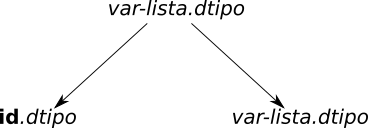
\includegraphics[scale=0.5]{figuras/exemplo67.png}
   \end{center}
   A regra gramatical $\textit{var-lista}\to\textbf{id}$ tem como grafo a ligação direta entre os dois atributos. As regras $\textit{tipo}\to\textbf{int}$ e $\textit{tipo}\to\textbf{float}$ são triviais, com atributos preenchidos pelas fases anteriores da compilação.
\end{frame}

\begin{frame}
   \frametitle{Construção do Grafo de Dependências}
   Para a regra gramatical:
   \begin{center}
   $\textit{decl} \to \textit{tipo }\textit{var-lista}$ 
   \end{center}
   temos a equação de atributos: 
   \begin{center}
   $\textit{var-lista}.dtipo = \textit{tipo}.dtipo$ 
   \end{center}
   o grafo de dependências tem o formato:
   \begin{center}
   $tipo.dtipo\longrightarrow  \textit{var-lista}.dtipo$ 
   \end{center}
   O problema é que, sem \textit{decl} visível, nós não sabemos qual regra origina o grafo. Podemos desenhar o grafo de dependência sobreposto a árvore de análise sintática para deixar claro qual regra define cada relação entre os atributos.
\end{frame}

\begin{frame}
   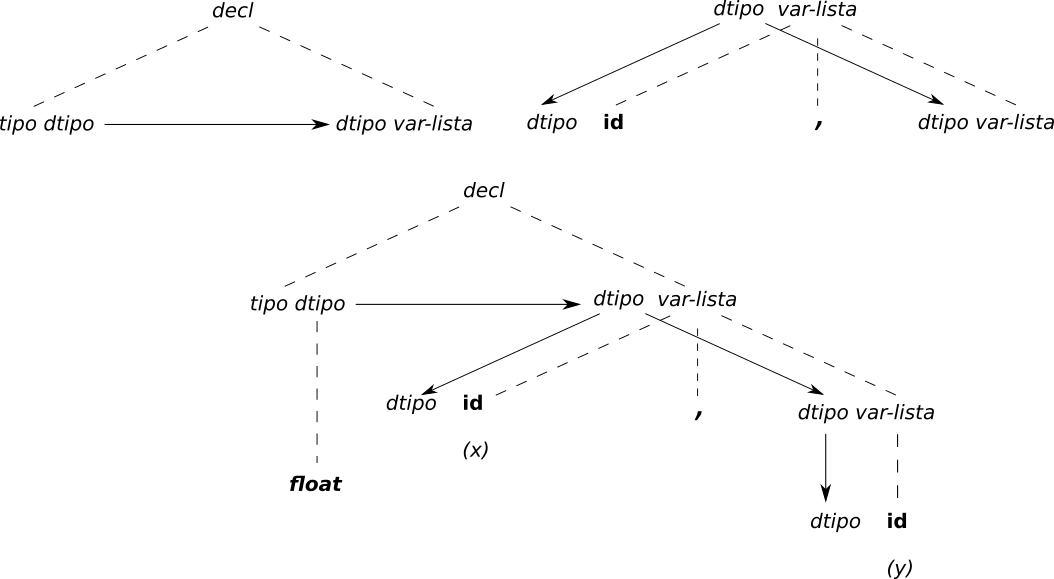
\includegraphics[width=\linewidth,height=\textheight,keepaspectratio]{figuras/exemplo67completo.png}
\end{frame}

\begin{frame}
   \frametitle{Construção do Grafo de Dependências}
   Na gramática para números octais e decimais, a regra $\textit{base-num}\to\textit{num basecar}$ tem as equações $\textit{base-num}.val = num.val$ e $num.base = basecar.base$. O detalhe importante para a construção do grafo é que agora são dois atributos.
   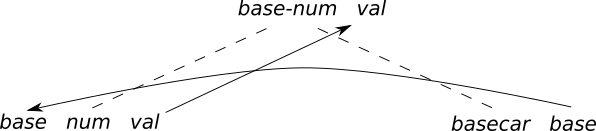
\includegraphics[width=\linewidth,height=\textheight,keepaspectratio]{figuras/exemplo68.png}
\end{frame}

\begin{frame}
   \frametitle{Construção do Grafo de Dependências}
   Regra $num \to num \textit{ dígito}$: \\
   \begin{center}
   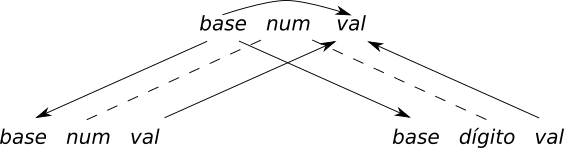
\includegraphics[scale=0.4]{figuras/exemplo68a.png}
   \end{center}
   \begin{columns}
   \begin{column}{0.5\textwidth}
   Regra $num \to \textit{dígito}$: \\
   \begin{center}
   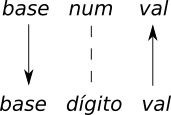
\includegraphics[scale=0.6]{figuras/exemplo68b.png}
   \end{center}
   \end{column}
   \begin{column}{0.5\textwidth}
   Regra $\textit{dígito} \to 9$: \\
   \begin{center}
   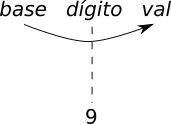
\includegraphics[scale=0.6]{figuras/exemplo68c.png}
   \end{center}
   \end{column}
   \end{columns}
   \begin{center}
   Como seria o grafo de dependências para 345o?
   \end{center}
\end{frame}

\begin{frame}
   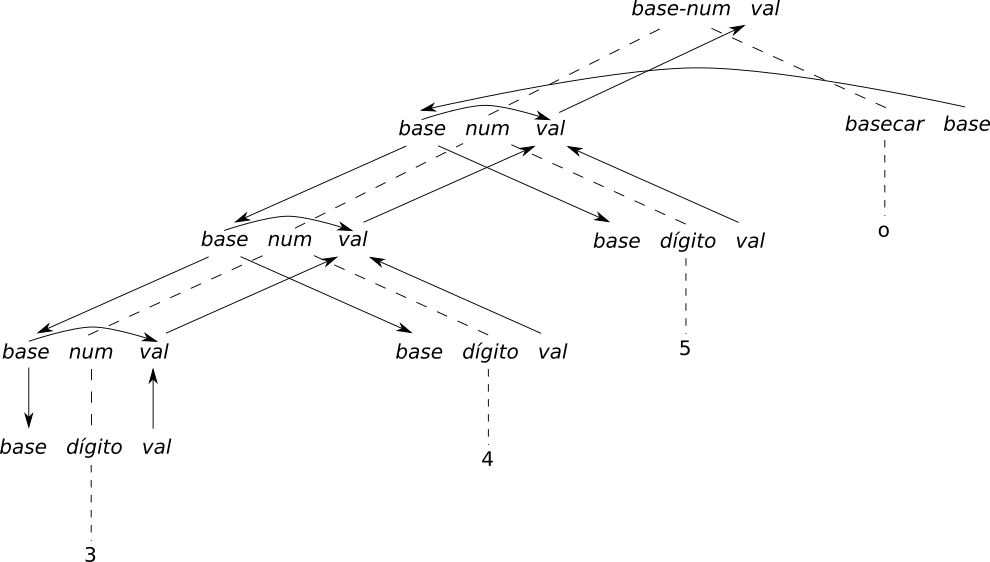
\includegraphics[width=\linewidth,height=\textheight,keepaspectratio]{figuras/exemplo68completo.png}
\end{frame}

\begin{frame}
   \frametitle{Algoritmos para Computação de Atributos}
   \begin{itemize}
      \item Qualquer algoritmo deve computar o atributo em cada nó no grafo antes de \textbf{tentar} computar atributos sucessores.
      \item \textbf{ordenação topológica}: percurso no grafo que obedece a restrição acima;
      \item só existem ordenações topológicas para \textbf{grafos direcionados acíclicos}, DAGs;
      \item uma \textbf{raiz} de um grafo é um nó sem predecessores.
   \end{itemize}
\end{frame}

\begin{frame}
   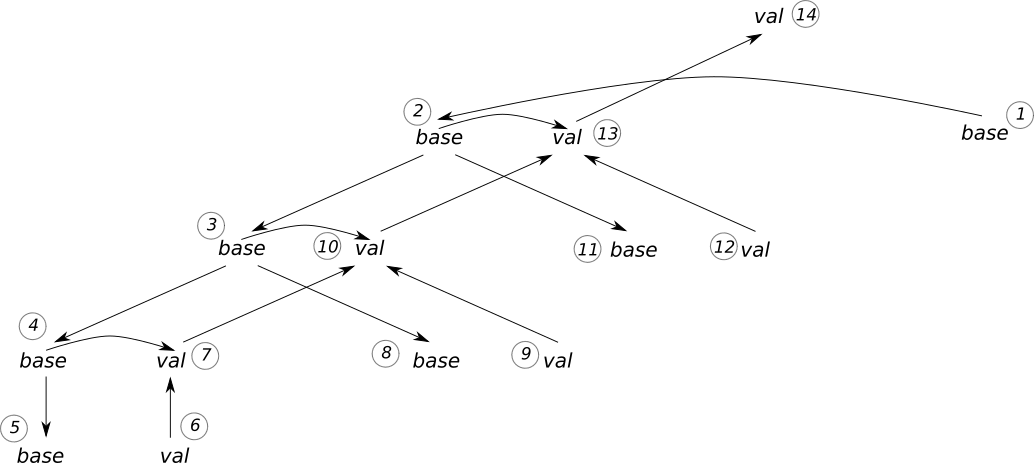
\includegraphics[width=\linewidth,height=\textheight,keepaspectratio]{figuras/exemplo68grafo.png}
\end{frame}

\begin{frame}
   \frametitle{Método de Árvore de Análise Sintática}
   \begin{itemize}
      \item Realizar a análise de atributos construindo um grafo de dependências e uma ordenação topológica;
      \item eficaz desde que a gramática de atributos não seja \textbf{circular};
      \item existem algoritmos para testar se uma gramática de atributos é circular ou não, em tempo exponencial;
      \item usando esses algoritmos, e técnicas para construção de ordenações topológicas, teríamos um gerador de analisadores semânticos;
      \item a maioria dos compiladores, entretanto, utiliza o \textbf{método baseado em regras}, ou seja, determinar através de código a ordem de avaliação dos atributos;
      \item é suficiente para gramáticas \textbf{fortemente não circulares}.
   \end{itemize}
\end{frame}

\begin{frame}
   \frametitle{Atributos Sintetizados}
   Para definir um método baseado em regras, seja percorrendo ou não a árvore sintática, precisamos estabelecer a natureza dos atributos. 
   \begin{block}{Definição}
   Todas as suas dependências apontarem de filho para pai na árvore de análise sintática. Atributo $a$ é sintetizado se dada uma regra $A\to X_{1}X_{2}...X_{n}$, a única equação de atributos associada com um $a$ a esquerda é da forma: \\
   \begin{center}
   $A.a = f(X_{1}.a_{1},...,X_{1}.a_{k},..., X_{n}.a_{1}, ..., X_{n}.a_{k})$ \\
   \end{center}
   Uma gramática de atributos em que todos os atributos são sintetizados é denominada \textbf{gramática S-atribuída}.
   \end{block}
\end{frame}

\begin{frame}[fragile]
   \frametitle{Como Programar o Cálculo de Atributos Sintetizados}
   Se a gramática de atributos for S-atribuída, podemos utilizar um percurso ascendente (pós ordem) na construção da árvore de análise sintática. 
   \begin{minted}{pascal}
   procedure Pós-Eval(T:nó-árvore);
   begin
      for cada filho C de T do
         Pós-Eval(C); 
      compute cada atributo sintetizado de T;
   end;
   \end{minted}
\end{frame}

\begin{frame}[fragile]
   \frametitle{Um Algoritmo para a Gramática de Atributos das Expressões Aritméticas}
   \begin{minted}{c}
   typedef enum {Plus, Minus, Times} OpKind;
   typedef enum {OpKind, ConstKind} ExpKind;
   typedef struct streenode {
      ExpKind kind;
      OpKind op;
      struct streenode *lchild, *rchild;
      int val;
   } STreeNode;
   typedef STreeNode *SyntaxTree;
   \end{minted}
\end{frame}

\begin{frame}[fragile]
   \frametitle{Um Algoritmo para a Gramática de Atributos das Expressões Aritméticas}
   \small
   \begin{minted}{c}
void postEval(SyntaxTree t) {
   int temp;
   if (t->kind == OpKind) {
      postEval(t->lchild);
      postEval(t->rchild);
      switch (t->op) {
         case Plus:
	    t->val = t->lchild->val + t->rchild->val;
	    break;
	 case Minus;
	    t->val = t->lchild->val - t->rchild->val;
	    break;
	 case Times;
	    t->val = t->lchild->val * t->rchild->val;
	    break;
      } /* end switch */
   } /* end if */
} /* end postEval */
   \end{minted}
\end{frame}

\begin{frame}
   \frametitle{Atributos Herdados}
   \begin{block}{Definição}
   \begin{itemize}
      \item Um atributo que não é sintetizado é denominado \textbf{herdado};
      \item os atributos herdados têm dependências que fluem de pai para filhos ou entre irmãos;
      \item a razão de chamar os dois casos de herança é porque a transmissão de atributos entre irmãos é geralmente implementada de modo que os valores dos atributos passam entre os irmãos através do pai.
   \end{itemize}
   \end{block}
   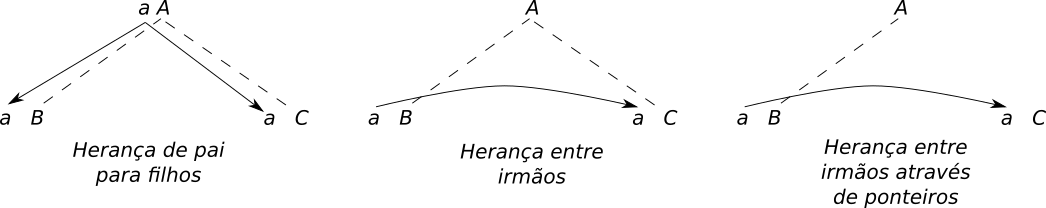
\includegraphics[width=\linewidth,height=\textheight,keepaspectratio]{figuras/exemplo69.png}
\end{frame}

\begin{frame}[fragile]
   \frametitle{Métodos Algorítmicos para Calcular Atributos Herdados}
   Percurso em pré-ordem, ou a combinação de pré-ordem e \textit{in}-ordem, para percorrer a árvore.
   \begin{minted}{pascal}
procedure Pré-Eval (T:nó-árvore);
begin
   for cada filho C de T do
      compute cada atributo herdado de C;
      Pré-Eval(C);
end;
   \end{minted}
   \begin{itemize}
      \item A ordem agora importa;
      \item a sequência de visitas na definição do \textbf{for};
      \item requisitos das dependências.
   \end{itemize}
\end{frame}

\begin{frame}[fragile]
   \frametitle{Métodos Algorítmicos para Calcular Atributos Herdados}
   Considerando novamente a gramática: \\
   $decl\to\textit{tipo var-lista}$ \\
   $tipo\to \textbf{int}|\textbf{float}$ \\
   $\textit{var-lista} \to \textbf{id},\textit{var-lista} | \textbf{id}$ \\
   \scriptsize
   \begin{minted}{pascal}
procedure AvalTipo(T:nó-arvore);
begin
   case tipo-nó de T of
   decl:
      AvalTipo(tipo);
      Atribui dtipo de tipo a dtipo de var-lista;
      AvalTipo(var-lista);
   tipo:
      if filho de T = int then T.dtipo := inteiro
      else T.dtipo := real;
   var-lista:
      atribui T.dtipo a primeiro filho de T;
      if terceiro filho de T não é nulo then
         atribui T.dtipo a terceiro filho;
	 AvalTipo(terceiro filho de T);
   end case;
end AvalTipo;
   \end{minted}
\end{frame}

\begin{frame}
   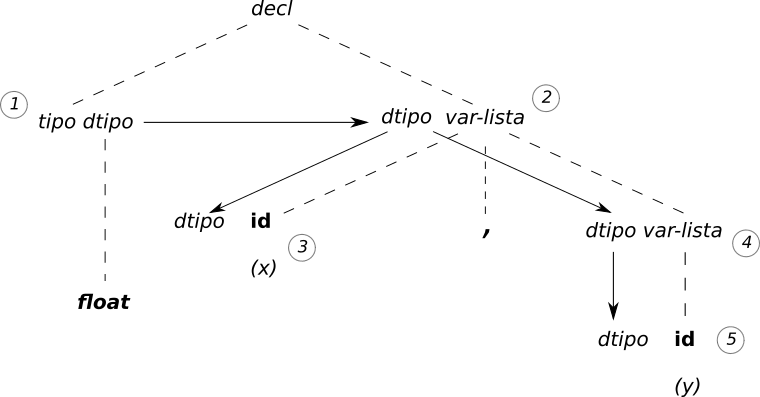
\includegraphics[width=\linewidth,height=\textheight,keepaspectratio]{figuras/exemplo610.png}
\end{frame}

\begin{frame}[fragile]
   \frametitle{Usando Árvores Sintáticas Simplificadas}
   Podemos representar \textit{var-lista} como uma lista encadeada de nós \textbf{id}. \\
   \begin{center}
   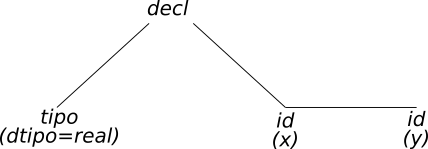
\includegraphics[scale=0.5]{figuras/exemplo610simplificado.png}
   \end{center}
   \begin{minted}{c}
   typedef enum {decl, type, id} nodekind;
   typedef enum {integer, real} typekind;
   typedef struct treeNode {
      struct treeNode *lchild, *rchild, *sibling;
      typekind dtype; /* para nós tipo e id */
      char *name;     /* apenas para nós id */
   } * SyntaxTree;
   \end{minted}
\end{frame}

\begin{frame}[fragile]
   \frametitle{Usando Árvores Sintáticas Simplificadas}
   \begin{minted}{c}
void evalType(SyntaxTree t) {
   switch (t->kind) {
      case decl:
         t->rchild->dtype = t->lchild->dtype;
	 evalType(t->rchild);
	 break;
      cade id:
         if (t->sibling != NULL) {
	    t->sibling->dtype = t->dtype;
	    evalType(t->sibling);
	 }
   } /* fim do switch */ 
} /* fim do AvalTipo */
   \end{minted}
\end{frame}

\begin{frame}
   \frametitle{Métodos Algorítmicos para Calcular Atributos}
   $\textit{base-num}\to\textit{num basecar}$ \\
   $basecar\to\textbf{o}|\textbf{d}$ \\
   $num\to\textit{num dígito}|\textit{dígito}$ \\ 
   $\textit{dígito}\to0|1|2|3|4|5|6|7|8|9$ \\
   \begin{itemize}
      \item Atributo sintetizado $val$ e atributo herdado $base$;
      \item $val$ depende de $base$;
      \item $base$ é herdado do filho direito para o filho esquerdo de um \textit{base-num};
      \item misturar métodos pré-ordem e pós-ordem.
   \end{itemize}
\end{frame}

\begin{frame}[fragile]
   \scriptsize
   \begin{columns}
   \begin{column}{0.5\textwidth}
   \begin{minted}{pascal}
procedure AvalComBase(T:árvore-nó):
begin
   case nó-tipo de T of
   base-num:
      AvalComBase(basecar);
      num.base := basecar.base;
      AvalComBase(num);
      T.val := num.val;
   num:
      filhoEsq := T.arvoreEsquerda;
      filhoEsq.base := T.base;
      AvalComBase(filhoEsq);
      filhoDir := T.arvoreDireita;
      if filhoDir não é nulo then
         filhoDir.base := T.base;
	 AvalComBase(filhoDir);
	 if (filhoDir.val != erro and 
	    filhoEsq.val != erro) then
	    T.val := T.base * 
	      (filhoEsq.val + filhoDir.val)
	 else T.val := erro;
      else T.val = filhoEsq.val;	   
  \end{minted}
   \end{column}
   \begin{column}{0.5\textwidth}
   \begin{minted}{pascal}
   basecar:
      if filho de T = o then 
         T.base := 8;
      else T.base := 10;
   dígito:
      if (T.base = 8 and (filho de T = 8 
         or filho de T = 9)) then
	 T.val := erro;
      else
         T.val := numval(filho de T);
   end case;	 
end AvalComBase;
   \end{minted}
   \end{column}
   \end{columns}
\end{frame}

\begin{frame}[fragile]
   \frametitle{Métodos Algorítmicos para Calcular Atributos}
   Nas gramáticas de atributos com sintetizados e herdados, sendo que os sintetizados dependem dos herdados, mas os herdados não dependem de sintetizados, é possível fazer o cálculo em uma única passada.
   \begin{minted}{pascal}
procedure CombinaEval(T:nó-árvore):
begin
   for cada filho C de T do
      compute cada atributo herdado de C;
      CombinaEval(C);
   compute cada atributo sintetizado de T;   
end;
   \end{minted}
   Situações nas quais atributos herdados dependem de sintetizados exigem mais de uma passada.
\end{frame}

\begin{frame}
   \frametitle{Métodos Algorítmicos para Calcular Atributos}
   Operações interpretadas de maneira diferente, se o número for ponto flutuante ou não. \\
   \begin{center}
   $S\to exp$ \\
   $exp\to exp/exp|\textbf{num}|\textbf{num.num}$
   \end{center}
   \begin{itemize}
      \item \textit{éFlut}: atributo booleano sintetizado;
      \item \textit{etipo}: atributo herdado, \textit{int} ou \textit{float};
      \item \textit{val}: atributo sintetizado.
   \end{itemize}
\end{frame}

\begin{frame}
   \frametitle{Métodos Algorítmicos para Calcular Atributos}
   \begin{table}
      \begin{tabular}{cc}
      Regra Gramatical & Regras Semânticas \\
      \hline 
      $S\to exp$ & exp.etipo = \textbf{if} exp.éflut \textbf{then} float \textbf{else} int \\
                 & S.val = exp.val \\      
      \hline
      $exp_{1}\to exp_{2}/exp_{3}$ & $\text{exp}_{1}.\text{éFlut} = \text{exp}_{2}.\text{éFlut} \textbf{ or } \text{exp}_{3}.\text{éFlut}$ \\ 
      & $\text{exp}_{2}.\text{etipo} = \text{exp}_{1}.\text{etipo}$ \\
      & $\text{exp}_{3}.\text{etipo} = \text{exp}_{1}.\text{etipo}$ \\
      & $\text{exp}_{1}.\text{val} = \textbf{if } \text{exp}_{1}.\text{etipo} = \text{int}$ \textbf{ then } \\
      & $\text{exp}_{2}.\text{val} \textbf{ div } \text{exp}_{3}.\text{val} $ \\
      & $\textbf{ else } \text{exp}_{2}.\text{val} / \text{exp}_{3}.\text{val} $ \\ 
      \hline
      $exp\to \textbf{num}$ & $\text{exp.éFlut} = \textbf{false}$ \\
      & exp.val = \textbf{if} exp.etipo = int \textbf{then} \textbf{num}.val \\
      & \textbf{else} Float(\textbf{num}.val) \\
      \hline
      $exp \to \textbf{num.num}$ & exp.éFlut = \textbf{true} \\
      & exp.val = \textbf{num.num}.val \\
      \end{tabular}
   \end{table}
\end{frame}

\begin{frame}
   \frametitle{Métodos Algorítmicos para Calcular Atributos}
   Duas passadas:
   \begin{itemize}
      \item A primeira passada computa o atributo sintetizado \textit{éFlut} em pós-ordem;
      \item A segunda passada computa o atributo herdado \textit{etipo} e o atributo sintetizado \textit{val} com um percurso combinado em pré-ordem e pós-ordem.
   \end{itemize}
   Como ficaria o cálculo de atributos para $5/2/2.0$?
\end{frame}

\begin{frame}
   \frametitle{Atributos como Parâmetros e Valores de Retorno}
   \begin{itemize}
      \item No lugar de preencher os valores em uma árvore, podemos transmitir os valores dos atributos como o valor de retorno dos procedimentos recursivos;
      \item Um único procedimento para percorrer a árvore:
      \begin{itemize}
         \item Computação dos atributos herdados em pré-ordem;
	 \item computação dos atributos sintetizados em pós-ordem;
	 \item transmitir os valores dos atributos herdados como parâmetros para ativações recursivas dos filhos;
	 \item receber valores dos atributos sintetizados como valores de retorno das ativações.
      \end{itemize}
      \item essa metodologia já foi demonstrada na gramática do cálculo de expressões;
      \item para atributos estruturados com maior complexidade, uma tabela de símbolos ou variáveis globais (\textbf{estruturas externas}) podem ser empregadas para manter valores entre as ativações.
   \end{itemize}
\end{frame}

\begin{frame}[fragile]
   \frametitle{Atributos como Parâmetros e Valores de Retorno}
   \scriptsize
   \begin{minted}{pascal}
function AvalComBase(T: no-arvore; base:inteiro): inteiro;
var temp, temp2: inteiro:
begin
      case no-tipo de T of
      base-num:
         temp := AvalComBase(filho a direita de T);
         return AvalComBase(filho a esquerda de T, temp);
      num:
         temp := AvalComBase(filho a esquerda de T, base);
         if filho a direita de T nao nil then
            temp2 := AvalComBase(filho a direita de T, base);
            if temp <> erro and temp2 <> erro then 
               return base * temp +  temp2;
            else return erro;
         else return temp;
      basecar:
         if filho de T = o then return 9
         else return 10;
      digito:
         if base = 8 and filho de T = 8 ou 9 then return erro
         else return numval(filho de T);
      end case;
end AvalComBase;
   \end{minted}
\end{frame}

\begin{frame}[fragile]
   \frametitle{Atributos como Parâmetros e Valores de Retorno}
   \begin{itemize}
      \item Funciona somente porque tanto \textit{base} quanto \textit{val} podem ser representados por inteiros;
      \item a primeira ativação seria \textit{AvalComBase(nó-raiz, 0);}
      \item uma possibilidade seria dividir a função em três.
   \end{itemize}
   \small
   \begin{minted}{pascal}
function AvalBaseNum(T: no-arvore): inteiro;
(* ativado apenas para a raiz *)            
begin
   return AvalNum(filho esquerdo de T, 
                  AvalBase(filho direito de T));
end AvalBaseNum
function AvalBase(T: no-arvore): inteiro;
(* ativado apenas para basecar *)            
begin
   if filho de T igual ao then return 8
   else return 10;
end AvalBase
\end{minted}
\end{frame}

\begin{frame}[fragile]
   \frametitle{Atributos como Parâmetros e Valores de Retorno}
   \scriptsize
   \begin{minted}{pascal}
function AvalNum(T: no-arvore): inteiro;
var temp, temp2: inteiro:
begin
      case no-tipo de T of
      num:
         temp := AvalComBase(filho a esquerda de T, base);
         if filho a direita de T nao nil then
            temp2 := AvalComBase(filho a direita de T, base);
            if temp <> erro and temp2 <> erro then 
               return base * temp +  temp2;
            else return erro;
         else return temp;
      digito:
         if base = 8 and filho de T = 8 ou 9 then return erro
         else return numval(filho de T);
      end case;
end AvalComBase;
   \end{minted}
   \normalsize
   O que essa separação quer mostrar é que o desenvolvedor do compilador tem liberdade para refatorar o código.
\end{frame}

\begin{frame}[fragile]
   \frametitle{Estruturas de Dados Externas}
   \begin{itemize}
      \item No exemplo anterior, seria realmente necessário a cópia de \textit{base} em vários argumentos?
      \item podemos supor a existência de estruturas de dados \textit{externas}:
      \begin{itemize}
         \item Variáveis globais;
         \item \textbf{tabelas}.
      \end{itemize}
   \end{itemize}
   \begin{minted}{pascal}
base-num:
      AjustaBase(filho direito de T);
      return AvalComBase(filho esquerdo de T);
   \end{minted}
   \begin{itemize}
      \item \textit{AjustaBase} seria um procedimento externo que configura uma variável global;
      \item todos os outros casos acessam essa variável;
      \item as regras semânticas podem ser atualizadas para refletir a variável global.
   \end{itemize}
\end{frame}

\begin{frame}[fragile]
   \frametitle{Estruturas de Dados Externas}
   Considerando a gramática de declaração de tipos, podemos ter o procedimento: \\
   \footnotesize
   \begin{minted}{pascal}
procedure inserir (nome: cadeia de caracteres; dtipo: tipo);
   \end{minted}
   \begin{table}
      \begin{tabular}{cc}
      Regra Gramatical & Regras Semânticas \\
      \hline 
      \textit{decl} $\rightarrow$ \textit{tipo var-lista} &  \\    
      \textit{tipo} $\rightarrow$ \textbf{int} & $dtipo = inteiro$ \\
      \textit{tipo} $\rightarrow$ \textbf{float} & $dtipo = real$ \\
      ${\text{var-lista}}_{1} \rightarrow \text{\textbf{id,}} {\text{var-lista}}_{2}$ & \textit{inserir(\textbf{id}.nome, dtipo)} \\
      $\text{var-lista} \rightarrow \text{\textbf{id}}$ & \textit{inserir(\textbf{id}.nome, dtipo)} \\
      \end{tabular}   
   \end{table}  
   \normalsize 
   Há uma tabela que armazena o mapeamento do nome ao tipo declarado.
\end{frame}

\begin{frame}[fragile]
   \frametitle{Estruturas de Dados Externas}
   \begin{minted}{pascal}
procedure AvalTipo (T: no-arvore);
begin
   case tipo-no de T of
   decl:
      AvalTipo(tipo filho de T);
      AvalTipo(var-lista filha de T);
   tipo:
      if filho de T = int then dtipo := inteiro
      else dtipo := real;
   var-lista:
      inserir(nome do primeiro filho de T, dtipo)
      if terceiro filho de T nao nil then
         AvalTipo(terceiro filho de T);
   end case;
end AvalTipo;
   \end{minted}
 \end{frame}

\begin{frame}
   \frametitle{Computação de Atributos Durante a Análise Semântica}+
   \begin{itemize}
      \item Uma questão fundamental é quanto dos atributos já podem ser calculados durante a análise sintática;
      \item como a maioria dos algoritmos de análise sintática processa a entrada da esquerda para a direita, o cálculo de atributos também segue essa direção;
      \item uma gramática de atributos na qual cada atributo, sintetizado ou herdado, pode ser calculado através de outros atributos que só ocorrem à esquerda na regra gramatical é dita \textbf{L-atribuída}.
      \item podemos acrescentar uma \textbf{pilha de valores} e explicitar as \textbf{ações semânticas} durante a análise LR;
      \item a maioria dos compiladores da atualidade não utilizam essa técnica, por sua vez usam mais de uma passada.
   \end{itemize}
\end{frame}

\section{A Tabela de Símbolos}
\begin{frame}
   \frametitle{A Tabela de Símbolos}
   \begin{itemize}
      \item É um atributo herdado;
      \item também tem relevância na análise sintática e no sistema de varredura;
      \item estrutura de dados com três operações:
      \begin{itemize}
         \item \textit{inserir}: armazenar informações fornecidas pelas declarações de nomes;
	 \item \textit{verificar}: recuperar informações de um nome previamente inserido;
	 \item \textit{remover}: invalidar uma informação.
      \end{itemize}
      \item tipos de dados, escopo e localização na memória.
   \end{itemize}
\end{frame}

\begin{frame}
   \frametitle{A Estrutura da Tabela de Símbolos}
   \begin{itemize}
      \item Na prática, a estrutura mais utilizada é um \textit{dicionário}, no qual você informa uma \textit{chave} e recebe um \textit{valor};
      \item Possíveis implementações:
      \begin{itemize}
         \item Listas lineares;
	 \item árvores de buscas;
	 \item tabelas \textit{hash} (mais utilizada. \textbf{Por quê?}).
      \end{itemize}
      \item o estudo avançado dessas estruturas é assunto das disciplinas de Estruturas de Dados.
   \end{itemize}
\end{frame}

\begin{frame}
   \frametitle{Tabelas \textit{Hash}}
   Uma matriz, cujas células são denominadas \textbf{repositórios}, indexada por um intervalo de inteiros, em geral de 0 até o tamanho da tabela menos 1.
   \begin{itemize}
      \item Um \textbf{função de \textit{hashing}} transforma a chave de busca em um valor inteiro dentro do intervalo de índices;
      \item \textbf{colisões} de \textit{hashing};
      \item \textbf{resolução de colisões}:
      \begin{itemize}
         \item endereçamento aberto;
	 \item encadeamento separado (repositório como lista linear).
      \end{itemize}
      \item o tamanho da tabela é fixado durante a construção do compilador;
      \item deve ser um número \textbf{primo}, pois melhora o comportamento da função \textit{hashing}.
   \end{itemize}
\end{frame}

\begin{frame}[fragile]
   \frametitle{Declarações}
   As declarações de variáveis, tipos, funções, etc (tudo que tem um nome) nas linguagens de programação afetam o comportamento e a implementação da tabela de símbolos.
   \begin{itemize}
      \item Declarações de constantes
      \begin{minted}{c} 
const int size = 199; 
      \end{minted}
      \item declarações de tipos
      \begin{minted}{c} 
typed struct Entry * EntryPtr; 
      \end{minted}
      \item declarações de variáveis
\begin{minted}{c}
int a,b[100];
\end{minted}
      \item declarações de procedimentos e funções.
\begin{minted}{c}
int hash(char *key) { return char[0] - '0'; }
\end{minted}
   \end{itemize}
   As declarações podem ser \textbf{explícitas} ou \textbf{implícitas}.
\end{frame}

\begin{frame}
   \frametitle{Declarações}
   \begin{itemize}
      \item É mais fácil usar uma única tabela de símbolos para todos os tipos de declarações;
      \item para linguagens modernas, é preferível associar tabelas de símbolos separadas por regiões do programa (procedimento ou função) e ligá-las segundo as regras semânticas;
      \item os atributos vinculados a cada nome variam de acordo com o tipo de declaração;
      \item por exemplo, os atributos de uma constante são diferentes dos atributos de uma variável.
   \end{itemize}
\end{frame}

\begin{frame}
   \frametitle{Atributos Vinculados a Nomes}
   \begin{block}{Declarações de Constantes}
   \begin{itemize}
      \item Associam valores a nomes;
      \item podem ser valores estáticos substituídos no texto durante a compilação;
      \item outra alternativa é vinculação dinâmica, como uma variável;
      \item \textbf{atribuição única} em ambos os casos.
   \end{itemize}
   \end{block}
   \begin{block}{Declarações de Tipos}
   \begin{itemize}
      \item Vinculam nomes a tipos pré-existentes;
      \item vamos falar mais sobre tipos adiante.
   \end{itemize}
   \end{block}
\end{frame}

\begin{frame}
   \frametitle{Atributos Vinculados a Nomes}
   \begin{block}{Declarações de Variáveis}
   \begin{itemize}
      \item Vincula nomes a tipos;
      \item outro atributo é o \textbf{escopo};
      \item alocação de memória;
      \item \textbf{duração} ou \textbf{tempo de vida} da alocação;
   \end{itemize}
   \end{block}
   \begin{block}{Declarações de Procedimentos}
   \begin{itemize}
      \item Vincula um nome a uma posição de memória na qual está o código do procedimento;
      \item parâmetros;
      \item tipo de retorno.
   \end{itemize}
   \end{block}
\end{frame}

\begin{frame}
   \frametitle{Regras de Escopo e Estruturas de Blocos}
   \begin{block}{Declarações Antes do Uso}
   Um nome deve ser declarado no texto de um programa antes de qualquer referência a ele. 
   \end{block}
   \begin{block}{Estrutura de Blocos}
   \begin{itemize}
      \item \textbf{Linguagem Estruturada em Blocos}: permite o aninhamento de blocos dentro de blocos e o escopo das declarações em um bloco é limitado à ele e aos blocos nele contidos.
      \item \textbf{Regra do Aninhamento mais Próximo}: dadas diversas declarações de um mesmo nome, a declaração que se aplica a uma referência é aquela no bloco de aninhamento mais próximo da referência.
   \end{itemize}
   \end{block}
\end{frame}

\begin{frame}[fragile]
   \frametitle{Escopos Aninhados}
   \begin{columns}
   \begin{column}{0.5\textwidth}
   \begin{minted}{c}
int i, j;

int f (int tamanho)
{
   char i, temp;
   ...
   {
      double j;
      ...
   }
   ...
   {
      char *j;
      ...
   }
}
   \end{minted}
   \end{column}
   \begin{column}{0.5\textwidth}
   \small
   \begin{itemize}
      \item A operação na tabela de símbolos \textit{inserir} não pode escrever por cima declarações anteriores;
      \item deve ocorrer uma ocultação temporária, para que a operação \textit{verificar} encontre apenas a declaração inserida mais recentemente para um nome;
      \item a solução é que a tabela de símbolo deve ter comportamento similar a uma \textit{pilha};
      \item como ficaria a tabela para o código ao lado?
   \end{itemize}
   \end{column}
   \end{columns}
\end{frame}

\begin{frame}
   \frametitle{Alternativas para Construção de Tabela}
   \begin{itemize}
      \item Construir uma nova tabela para cada escopo;
      \item fazer a ligação das tabelas em uma lista, do escopo mais interno para o mais externo;
      \item a operação \textit{verificar} percorre a lista até encontrar o nome buscado;
      \item as regras de resolução de escopo podem ser ignoradas utilizando um \textbf{operador de resolução}.
   \end{itemize}
\end{frame}

\begin{frame}[fragile]
   \frametitle{Escopo Estático \textit{versus} Escopo Dinâmico}
   \begin{columns}
   \begin{column}{0.5\textwidth}
   \begin{minted}{c}
#include <stdio.h>

int i = 1;

void f(void) {
   printf("%d\n", i);
}

void main(void) {
   int i = 2;
   f();
   return 0;
}
   \end{minted}
   \end{column}
   \begin{column}{0.5\textwidth}
   \begin{itemize}
      \item Estamos concentrando nossas discussões no escopo estático, pois é o mais utilizado;
      \item nesse caso, a tabela de símbolos é construída em sua maior parte durante a compilação;
      \item o escopo dinâmico exige que tabela seja construída durante a execução.
   \end{itemize}
   \end{column}
   \end{columns}
\end{frame}

\begin{frame}[fragile]
   \frametitle{Interação em Declarações de Mesmo Nível}
   \begin{itemize}
      \item Para a maioria das linguagens, nomes não podem ser repetidos no mesmo escopo:
      \begin{minted}{c}
      typedef int i;
      int i;
      \end{minted}
      \item declaração sequêncial:
      \begin{minted}{c}
      int i = 2, j = i + 1;
      \end{minted}
      \item algumas linguagens funcionais adotam a declaração \textbf{colateral}, o oposto da sequêncial;
      \item declaração recursiva:
      \begin{minted}{c}
      int gcd(int n, int m) {
        if (m == 0) return n;
	else return gcd(m, n % m);
      }	
      \end{minted}
      \item o uso de protótipos de funções ameniza os problemas da recursão.
   \end{itemize}
\end{frame}

\begin{frame}
   \frametitle{Exemplo de Gramática de Atributos para Construção da Tabela de Símbolos}
   $S\to exp$ \\
   $exp\to(exp)|exp + exp|\textbf{id}|\textbf{num}|\textbf{let } \textit{dec-lista} \textbf{ in } exp$ \\
   $\textit{dec-lista} \to \textit{dec-lista}, decl | decl$ \\
   $decl\to \textbf{id}=exp$ \\
   \vspace{1.0cm}
   
   As declarações após a marca \textbf{let} estabelecem os nomes para expressões, os quais, quando aparecem na \textit{exp} após a marca \textbf{in}, substituem os valores. Em outras palavras, as expressões \textit{let} representam os blocos dessa linguagem.
\end{frame}

\begin{frame}[fragile]
   \frametitle{Exemplo de Gramática de Atributos para Construção da Tabela de Símbolos}
   \begin{minted}{haskell}
   -- Expressões Corretas
   let x = 2 + 1, y = 3 + 4 in x + y
   let x = 2, y = 3 in
      (let x = x + 1, y = (let z = 3 in x + y + z)
           in (x + y))
   -- Não pode haver redeclaração - Errado!
   let x = 2, x = 3 in x + 1
   -- Um nome precisa ser declarado - Errado!
   let x = 2 in x + y
   -- Aninhamento mais próximo
   let x = 2 in (let x = 3 in x)
   -- Declaração seqüêncial
let x = 2, y = x + 1 in (let x = x + y, y = x + y in y)
   \end{minted}
\end{frame}

\begin{frame}
   \frametitle{Objetivos da Tabela de Símbolos para o Exemplo}
   \begin{itemize}
      \item Vamos usar a tabela para determinar se uma expressão é errônea;
      \item atributo booleano sintetizado \textit{err} (\textbf{true} expressão errada, \textbf{false} caso contrário);
      \item atributo herdado \textit{simtab} para representar a tabela;
      \item atributo herdado \textit{nivelaninh}, para identificar o nível do bloco;
      \item $inserir(s, n, l)$ retorna uma nova tabela de símbolos que contém todas as informações de $s$, mas com o nome $n$ associado ao nível $l$;
      \item $estaem(s,n)$ verdadeiro ou falso se $n$ está em $s$ ou não;
      \item $verificar(s,n)$ retorna o aninhamento de $n$ em $s$.
   \end{itemize}
\end{frame}

\begin{frame}
   \frametitle{Gramática de Atributos para Tabela de Símbolos}
   \begin{table}
      \begin{tabular}{cc}
      Regra Gramatical & Regras Semânticas \\
      \hline 
      $S\to exp$ & $exp.simtab = tabelavazia$ \\
                 & $exp.nivelaninh = 0$ \\
                 & $S.err = exp.err$ \\
      \hline
      $exp_{1}\to exp_{2} + exp_{3}$ & $exp_{2}.simtab=exp_{1}.simtab$ \\
                                     & $exp_{3}.simtab=exp_{1}.simtab$ \\
                                     & $exp_{2}.nivelalinh=exp_{1}.nivelalinh$ \\
                                     & $exp_{3}.nivelalinh=exp_{1}.nivelalinh$ \\
                                     & $exp_{1}.err=exp_{2}.err \textbf{ or }exp_{3}.err$ \\
      \hline
      $exp_{1}\to(exp_{2})$ & $exp_{2}.simtab = exp_{1}.simtab$ \\
                            & $exp_{2}.nivelalinh = exp_{1}.nivelalinh$ \\
                            & $exp_{1}.err = exp_{2}.err$ \\
      \hline
      $exp\to\textbf{id}$ & $exp.err = \textbf{not } estaem(exp.simtab.\textbf{id}.nome)$ \\
      \hline
      $exp\to\textbf{num}$ & $exp.err = \textbf{false}$ \\
      \end{tabular}
   \end{table}
\end{frame}

\begin{frame}
   \frametitle{Gramática de Atributos para Tabela de Símbolos}
   \scriptsize
   \begin{table}
      \begin{tabular}{cc}
      Regra Gramatical & Regras Semânticas \\
      \hline
      $exp_{1}\to \textbf{ let } \textit{dec-lista} \textbf{ in } exp _{2}$ & $\textit{dec-lista}.enttab = exp_{1}.simtab$ \\
                                     & $\textit{dec-lista}.nivelalinh=exp_{1}.nivelalinh + 1$ \\
                                     & $exp_{2}.simtab=\textit{dec-lista}.saitab$ \\
                                     & $exp_{2}.nivelalinh=\textit{dec-lista}.nivelalinh$ \\
                                     & $exp_{1}.err=(\textit{decl-lista}.saitab = errtab) \textbf{ or }exp_{2}.err$ \\
      \hline
     $\textit{decl-lista}_{1}\to\textit{dec-lista}_{2}, decl$ & $\textit{dec-lista}_{2}.enttab = \textit{dec-lista}_{1}.enttab$ \\
                                                      & $\textit{dec-lista}_{2}.nivelalinh = \textit{dec-lista}_{1}.nivelalinh$ \\
                                                      & $\textit{decl}.enttab = \textit{dec-lista}_{2}.saitab$ \\
                                                      & $\textit{decl}.nivelalinh = \textit{dec-lista}_{2}.nivelalinh$ \\
                                                      & $\textit{decl-lista}_{1}.saitab = \textit{decl}.saitab$ \\
      \hline
      $\textit{decl-lista} \to decl$ & $decl.enttab = \textit{dec-lista}.enttab$ \\
                                     & $decl.nivelalinh = \textit{dec-lista}.nivelalinh$ \\
                                     & $\textit{dec-lista}.saitab = decl.saitab$ \\
      \end{tabular}
   \end{table}
\end{frame}

\begin{frame}
   \frametitle{Gramática de Atributos para Tabela de Símbolos}
   \small
   \begin{table}
      \begin{tabular}{cc}
      Regra Gramatical & Regras Semânticas \\
      \hline 
      $decl \to \textbf{id}=exp$ & $exp.simtab = decl.enttab$ \\
      & $exp.nivelalinh = decl.nivelalinh$ \\
      & $decl.saitab =$ \\
      & $  \textbf{if } (decl.enttab = errtab) \textbf{ or } exp.err $ \\
      & $  \textbf{then } errtab$ \\
      & $  \textbf{else if } (verificar(decl.enttab,\textbf{id}.nome) = decl.nivelaninh$ \\
      & $  \textbf{then } errtab$ \\
      & $  \textbf{else } insert(decl.enttab,\textbf{id}.nome, decl.nivelaninh)$ \\
      \end{tabular}
   \end{table}
\end{frame}

\section{Tipos de Dados e Verificações de Tipos}
\begin{frame}
   \frametitle{Tipos de Dados e Verificações de Tipos}
   \begin{block}{Inferência de Tipos}
   Computar e manter informações sobre tipos de dados de acordo com as declarações.
   \end{block}
   \begin{block}{Verificação de Tipos}
   Garantir que cada parte de um programa faça sentido para as regras de tipo da linguagem.
   \end{block}
   \begin{itemize}
      \item Em geral, chamamos as duas tarefas apenas de \textbf{verificação de tipos};
      \item informações estáticas sobre tipos:
      \begin{itemize}
         \item quantidade de memória requerida;
	 \item forma de acesso da memória.
      \end{itemize}
   \end{itemize}
\end{frame}

\begin{frame}[fragile]
   \frametitle{Tipos de Dados e Verificações de Tipos}
   \begin{block}{Tipos de Dados}
   É um conjunto de valores ou, mais precisamente, um conjunto de valores com certas operações sobre esses valores.
   \end{block}
   \begin{itemize}
      \item O tipo \textbf{int}, representa o conjunto de valores inteiros, nos quais podemos executar operações aritméticas;
      \item expressões de tipos:
      \begin{minted}{c}
// Apenas um nome de tipo
int a, b, c;
// Expressão estruturada
int vetor[100];
// Definição de novo tipo
typedef int notas[100];
      \end{minted}
   \end{itemize}
\end{frame}

\begin{frame}[fragile]
   \frametitle{Tipos de Dados e Verificações de Tipos}
   \begin{itemize}
      \item As informações de tipo podem ser explícitas, como nos exemplo em C;
      \item ou implícitas nas linguagens dinâmicas como Python:
      \begin{minted}{python}
universidade = "UFC Quixadá"
      \end{minted}
      \item considerando a linguagem C, a referência:
      \begin{minted}{c}
      a[i]
      \end{minted}
      \item os tipos de dados de $a$ e $i$ são recuperados da tabela de símbolos;
      \item se $a$ for do tipo $double []$ e $i$ for $int$, a subexpressão $a[i]$ será do tipo $double$;
   \end{itemize}
\end{frame}

\begin{frame}
   \frametitle{Expressões de Tipos e Construtores de Tipos}
   \begin{itemize}
      \item Os tipos \textbf{predefinidos} ou \textbf{primitivos} correspondem a tipos de dados numéricos fornecidos internamente por diversas arquiteturas de máquinas, como $int$, $double$, etc;
      \item os \textbf{construtores de tipos} como $typedef$ ou $struct$ podem ser vistos como funções que tomam tipos existentes como parâmetro e retornam novos tipos;
      \item são os chamados \textbf{tipos estruturados};
      \item um construtor de tipos corresponde a uma operação de conjuntos sobre os conjuntos subjacentes de valores dos seus parâmetros.
   \end{itemize}
\end{frame}

\begin{frame}[fragile]
   \frametitle{Expressões de Tipos e Construtores de Tipos}
   \begin{block}{Matrizes ou Vetores}
   Dois parâmetros de tipos: \textbf{tipo de índice} e \textbf{tipo de componente}.
   $ \textit{tipo componente } \text{vetor}[\textit{tipo índice}];$
   \begin{itemize}
      \item Na maioria das linguagens, o tipo de índice deve pertencer ao conjunto de \textbf{tipos ordinais};
      \item uma matriz representa valores que são sequências de valores do tipo componente, indexados pelos valores do tipo do índice;
      \item tipo índice com conjunto de valores $I$ e o tipo componente com valores $C$: um vetor é o conjunto de funções $I\to C$.
      \item matrizes multidimensionais: deteminadas pela \textbf{coluna} ou pela \textbf{linha};
      \item a tabela pode ter apenas o endereço inicial e o tipo componente, ou também incluir o tamanho.
   \end{itemize}
   \end{block}
\end{frame}

\begin{frame}[fragile]
   \frametitle{Expressões de Tipos e Construtores de Tipos}
   \begin{block}{Registros}
   Recebe uma lista de nomes e tipos associados e constrói um novo tipo.
   \begin{minted}{c}
struct {
   double r;
   int i;
}
   \end{minted}
   \begin{itemize}
      \item Para o exemplo acima, o registro corresponde a $(\textbf{r}xR)x(\textbf{i}xI)$ onde $r$ e $i$ representam o espaço de nomes possíveis, enquando $R$ e $I$ representam todos valores possíveis reais e inteiros;
      \item o registro é em geral alocado em sequência na memória;
      \item na tabela, entram o endereço inicial e o tipo de cada membro.
   \end{itemize}
   \end{block}
\end{frame}

\begin{frame}[fragile]
   \frametitle{Expressões de Tipos e Construtores de Tipos}
   \begin{block}{União}
   Corresponde à operação de união dos conjuntos de valores possíveis.
   \begin{minted}{c}
union {
   double r;
   int i;
}
   \end{minted}
   \begin{itemize}
      \item aloca-se o espaço necessário para o maior membro, nele se armazena o valor, seja acessado como inteiro ou real;
      \item a representação em \textit{bytes} do inteiro é diferente da representação real;
      \item $(\textbf{r}xR)\cup(\textbf{i}xI)$;
      \item a tabela tem que guardar o endereço da memória e uma lista de tipos possíveis.
   \end{itemize}
   \end{block}
\end{frame}

\begin{frame}[fragile]
   \frametitle{Expressões de Tipos e Construtores de Tipos}
   \begin{block}{Ponteiro}
   O valor de um tipo ponteiro é um endereço de memória.
   \begin{itemize}
      \item o espaço ocupado depende da arquitetura;
      \item se a linguagem permitir aritmética de ponteiros, a tabela tem que guardar, além do endereço, o tamanho do tipo do ponteiro, para saber quantos \textit{bytes} devem ser avançados por vez;
      \item a operação básica do tipo ponteiro é  \textbf{derreferenciação}.
   \end{itemize}
   \end{block}
\end{frame}

\begin{frame}[fragile]
   \frametitle{Expressões de Tipos e Construtores de Tipos}
   \begin{block}{Função}
   A função é um bloco de código invocável.
   \begin{itemize}
      \item a tabela precisa guardar o endereço onde começa o código da função;
      \item o tipo do valor de retorno;
      \item a lista de argumentos e seus tipos.
   \end{itemize}
   \end{block}
   \begin{block}{Classe}
   Similar a registros, porém com funções membro ou \textbf{métodos}.
   \begin{itemize}
      \item em linguagens orientadas à objetos, uma classe pode definir um novo tipo;
      \item a tabela armazena o endereço de um objeto, que deve ter sua memória organizada de acordo com o tipo definido pela classe;
   \end{itemize}
   \end{block}
\end{frame}

\begin{frame}[fragile]
   \frametitle{Nomes de Tipos, Declarações e Tipos Recursivos}
   \begin{minted}{c}
// Declaração de tipo em C
typedef struct {
   double r;
   int i;
} RealIntRec;
// Declaração detalhada
struct RealIntRec {
   double r;
   int i;
};
typedef struct RealIntRec RealIntRec;
   \end{minted}
   As declarações de tipos levam os nomes de tipos declarados a serem fornecidos na tabela de símbolos.
\end{frame}

\begin{frame}[fragile]
   \frametitle{Nomes de Tipos, Declarações e Tipos Recursivos}
   \begin{minted}{c}
// Declaração de tipo ilegal em C
struct intBST {
   int isNull;
   int val;
   struct intBST left, right;
};
// Declaração válida 
struct intBST {
   int val;
   struct intBST *left, *right;
};
typedef struct intBST * intBST;
   \end{minted}
   É importante lembrar que ponteiros sempre ocupam o mesmo espaço na memória.
\end{frame}

\begin{frame}[fragile]
   \frametitle{Equivalência de Tipos}
   \begin{block}{Motivação}
   Dadas as expressões possíveis de tipos de uma linguagem, um \textit{verificador de tipos} deve responder se duas expressões de tipos representam o mesmo tipo.
   \end{block}
   Imagine uma função:
   \begin{minted}{pascal}
function tipoIgual(t1, t2: TipoExp): Booleano;
   \end{minted}
   Recebe duas árvores, que representam derivações de expressões de uma gramática de linguagem, e retorna se ambas expressões são do mesmo tipo.
\end{frame}

\begin{frame}
   \frametitle{Equivalência de Tipos}
   $\textit{var-decls}\to \textit{var-decls}\textbf{;}\textit{var-decl}|\textit{var-decl}$ \\
   $\textit{var-decl}\to \textbf{id:}\textit{tipo-exp}$ \\
   $\textit{tipo-exp}\to \textit{tipo-simples}|\textit{tipo-estruturado}$ \\
   $\textit{tipo-simples}\to \textbf{int}|\textbf{bool}|\textbf{real}|\textbf{char}|\textbf{void}$ \\
   $\textit{tipo-estruturado}\to \textbf{array [num] of } \textit{tipo-exp }$ \\
   $|\textbf{record} \textit{ var-decls } \textbf{end}$ \\
   $|\textbf{union} \textit{ var-decls } \textbf{end}$ \\
   $|\textbf{pointer to} \textit{ tipo-exp}$ \\
   $|\textbf{proc } (\textit{tipo-exps}) \textit{ tipo-exp}$ \\
   $\textit{tipo-exps}\to \textit{tipo-exps}\textbf{,}\textit{tipo-exp}|\textit{tipo-exp}$
\end{frame}

\begin{frame}[fragile]
   \frametitle{Equivalência de Tipos}
   \begin{columns}
   \begin{column}{0.5\textwidth}
   \begin{minted}{pascal}
record
  x: pointer to real;
  y: array [10] of int
end
   \end{minted}
   \end{column}
   \begin{column}{0.5\textwidth}
   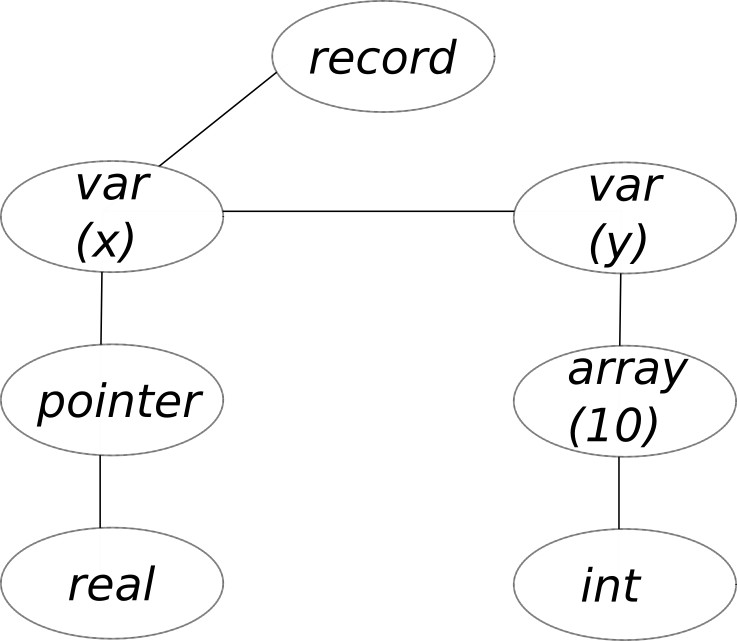
\includegraphics[width=\linewidth,height=\textheight,keepaspectratio]{figuras/record.png}
   \end{column}
   \end{columns}
\end{frame}

\begin{frame}[fragile]
   \frametitle{Equivalência de Tipos}
   \begin{minted}{pascal}
proc(bool, union a:real; b:char end, int):void   
   \end{minted}
   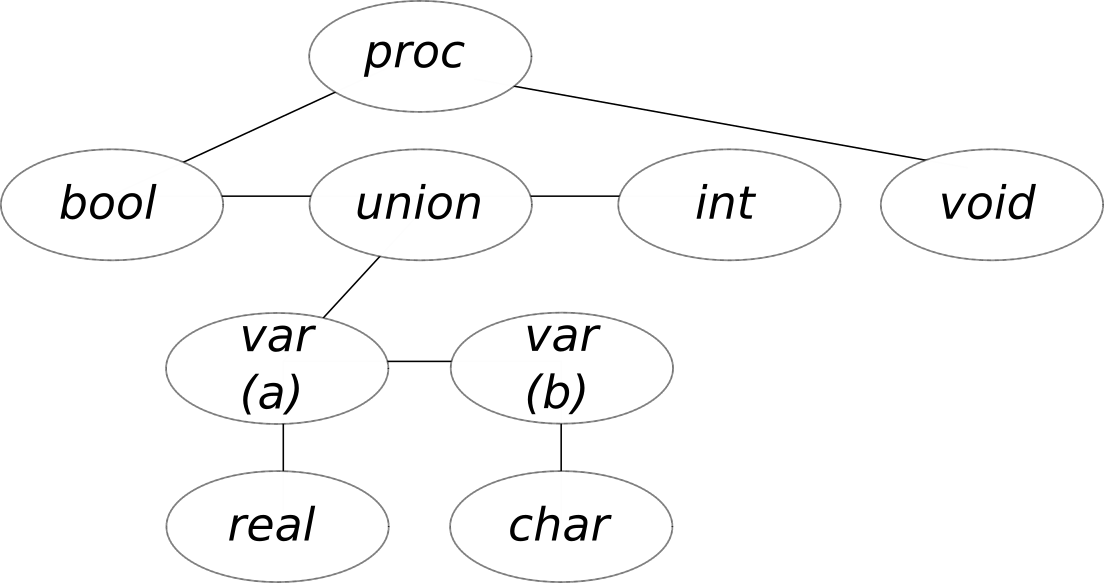
\includegraphics[width=\linewidth,height=\textheight,keepaspectratio]{figuras/proc.png}
\end{frame}

\begin{frame}
   \frametitle{Equivalência de Tipos}
   \begin{block}{Equivalência Estrutural}
   Dois tipos são iguais se e somente se tiverem a mesma estrutura.
   \begin{itemize}
      \item Em termos de árvores, dois tipos são equivalente se suas árvores tiverem a mesma \textbf{estrutura};
      \item os atributos em cada nó das árvores podem ser diferentes.
   \end{itemize}
   \end{block}
\end{frame}

\begin{frame}[fragile]
   \frametitle{Equivalência de Tipos}
   \tiny
   \begin{columns}
   \begin{column}{0.5\textwidth}
   \begin{minted}{pascal}
function tipoIgual (t1, t2:TipoExp):Booleano;   
var temp:Booleano;
    p1, p2:TipoExp;
begin
   if t1 e t2 são de tipos simples then 
      return t1 = t2
   else if (t1.tipo = matriz 
             and t2.tipo = matriz) then   
      return (t1.tamanho = t2.tamanho 
             and tipoIgual(t1.filho1, t2.filho1))
   else if ((t1.tipo = registro 
             and t2.tipo = registro)
	     or (t1.tipo = uniao 
	     and t2.tipo = uniao)) then
   begin
      p1 := t1.tipo1;
      p2 := t2.tipo1;
      temp := true;
      while temp and p1 != nil and p2 != nil do
         if p1.nome != p2.nome then
	    temp := false
	 else if not tipoIgual(p1.filho1, p2.filho1)
	 then temp := false
	 else begin
	   p1 := p1.irmão;
	   p2 := p2.irmão;
	 end;
      return temp and p1 = nil and p2 = nil;
   end
   \end{minted}
   \end{column}
   \begin{column}{0.5\textwidth}
   \begin{minted}{pascal}
   else if (t1.tipo = ponteiro 
            and t2.tipo = ponteiro) then
      return tipoIgual(t1.filho1, t2.filho1)   
   else if (t1.tipo = proc and t2.tipo = proc) then
   begin
      p1 := t1.filho1;
      p2 := t2.filho1;
      temp := true;
      while temp and p1 != nil and p2 != nil do
         if not tipoIgual(p1.filho1, p2.filho1)
	 then temp := false
	 else begin
	   p1 := p1.irmão;
	   p2 := p2.irmão;
	 end;
      return temp and p1 = nil and p2 = nil 
             and tipoIgual(t1.filho2, t2.filho2)
   end
   else return false;
end; (* tipoIgual *)
   \end{minted}
   \end{column}
   \end{columns}
\end{frame}

\begin{frame}
   \frametitle{Equivalência de Tipos}
   Uma alteração na gramática para permitir novos nomes para tipos: \\
   $\textit{var-decls}\to \textit{var-decls}\textbf{ ; }\textit{var-decl}|\textit{var-decl}$ \\
   $\textit{var-decl}\to \textbf{id : }\textit{exp-tipo-simples}$ \\
   $\textit{tipo-decls}\to \textit{tipo-decls}\textbf{ : } \textit{tipo-decl}|\textit{tipo-decl}$ \\
   $\textit{tipo-decl}\to \textbf{id = }\textit{tipo-exp}$ \\
   $\textit{tipo-exp}\to \textit{exp-tipo-simples}|\textit{tipo-estruturado}$ \\
   $\textit{exp-tipo-simples}\to \textit{tipo-simples}|\textbf{id}$ \\
   $\textit{tipo-simples}\to \textbf{int}|\textbf{bool}|\textbf{real}|\textbf{char}|\textbf{void}$ \\
   $\textit{tipo-estruturado}\to \textbf{array [num] of } \textit{tipo-exp }$ \\
   $|\textbf{record} \textit{ var-decls } \textbf{end}$ \\
   $|\textbf{union} \textit{ var-decls } \textbf{end}$ \\
   $|\textbf{pointer to} \textit{ tipo-exp}$ \\
   $|\textbf{proc } (\textit{tipo-exps}) \textit{ tipo-exp}$ \\
   $\textit{tipo-exps}\to \textit{tipo-exps}\textbf{,}\textit{exp-tipo-simples}|\textit{exp-tipo-simples}$
\end{frame}

\begin{frame}[fragile]
   \frametitle{Equivalência de Tipos}
   No lugar de:
   \begin{minted}{pascal}
record 
   x: pointer to real;
   y: array [10] of int
end
   \end{minted}
   precisamos ter:
   \begin{minted}{pascal}
   t1 = pointer to real;
   t2 = array [10] of int;
   t3 = record
           x: t1;
	   y: t2
   end
   \end{minted}
   \textbf{Equivalência de Nomes}: duas expressões de tipos são equivalentes se e somente se forem o mesmo tipo simples ou o mesmo nome de tipo.
\end{frame}

\begin{frame}[fragile]
   \frametitle{Equivalência de Tipos}
   \begin{minted}{pascal}
function tipoIgual(t1,t2: TipoExp): Booleano;
var temp: Booleano;
    p1, p2: TipoExp;
begin
   if t1 e t1 são de tipos simples then
      return t1 = t2
   else if t1 e t2 são nomes de tipos then
      return t1 = t2
   else return falso;
end;
   \end{minted}
\end{frame}

\begin{frame}
   \frametitle{Equivalência de Tipos}
   \begin{itemize}
      \item A \textbf{equivalência estrutural} tem alta complexidade;
      \item a \textbf{equivalência de nomes} é muito restrita;
      \item \textbf{equivalência de declarações}:
      \begin{itemize}
         \item cada nome é equivalente a um nome básico ou a uma expressão de tipos;
	 \item toda expressão de tipos é cadastrada na tabela de símbolos;
	 \item novos nomes que utilizam a mesma expressão apontam para a mesma entrada na tabela.
      \end{itemize}
      \item a tabela de símbolos deve oferecer uma nova operação \textit{capturaNomeBaseTipo}.
   \end{itemize}
\end{frame}

\begin{frame}[fragile]
   \frametitle{Equivalência de Tipos}
   Considere, para equivalência de declarações:
   \begin{minted}{pascal}
t1 = array [10] of int;
t2 = array [10] of int;
t3 = t1;
   \end{minted}
   Tanto $t1$ quanto $t2$ e $t3$ apontam para a entrada na tabela de \textit{array [10] of int}. O compilador precisa, para cada expressão de tipos, verificar se a mesma já existe na tabela.
\end{frame}

\begin{frame}
   \frametitle{Inferência e Verificação de Tipos}
   Considerando que temos:
   \begin{itemize}
      \item Uma operação \textit{tipoIgual} que retorna verdadeiro ou falso;
      \item uma operação de \textit{inserir} na tabela de símbolos;
      \item uma operação de \textit{verificar} na tabela de símbolos.
   \end{itemize}
   Vamos simplificar a gramática para: \\
   \textit{programa} $\to$ \textit{var-decls} \textbf{;} \textit{decls} \\
   \textit{var-decls} $\to$ \textit{var-decls} \textbf{;} \textit{var-decl} $|$ \textit{var-decl} \\
   \textit{var-decl} $\to$ \textbf{id :} \textit{tipo-exp} \\
   \textit{tipo-exp} $\to$ \textbf{int} $|$ \textbf{bool} $|$ \textbf{array [num] of} \textit{tipo-exp} \\
   \textit{decls} $\to$ \textit{decls} \textbf{;} \textit{decl} $|$ \textit{decl} \\
   \textit{decl} $\to$ \textbf{if} \textit{exp} \textbf{then} \textit{decl} $|$ \textbf{id :} \textit{exp} \\
   Vamos definir uma gramática de atributos que verifique se as expressões estão corretas de acordo com o sistema de tipos.
\end{frame}

\begin{frame}
   \frametitle{Inferência e Verificações de Tipos}
   \begin{table}
      \begin{tabular}{c|c}
      \textbf{Regra Gramatical} & \textbf{Regras Semânticas} \\
      \hline
      \hline
      \textit{var-decl} $\to$ \textbf{id :} \textit{tipo-exp} & $inserir(\textbf{id}.nome, \textit{tipo-exp}.tipo)$ \\
      \hline
      \textit{tipo-exp} $\to$ \textbf{int} & \textit{tipo-exp.tipo} := \textit{inteiro} \\
      \hline
      \textit{tipo-exp} $\to$ \textbf{bool} & \textit{tipo-exp.tipo} := \textit{booleano} \\
      \hline
      $\textit{tipo-exp}_{1}\to$ & $\textit{tipo-exp}_{1}.tipo$ :=  \\
      \textbf{array[num] of} $\textit{tipo-exp}_{2}$ & criaTipoNó(matriz,\\
      & \textbf{num}.tamanho,$\textit{tipo-exp}_{2}$.tipo) \\
      \hline
      \textit{decl} $\to$ \textbf{if} \textit{exp} \textbf{then} \textit{decl} & \textbf{if not} \textit{tipoIgual}(\textit{exp.tipo, booleano}) \\
      & \textbf{then} \textit{tipo-erro(decl)} \\
      \hline
      \textit{decl} $\to$ \textbf{id :=} \textit{exp} & \textbf{if not} \textit{tipoIgual}(\textit{verificar(\textbf{id}.nome})\\
      & , \textit{exp.tipo}) \textbf{then} \textit{tipo-erro(decl)} \\
      \hline
      \end{tabular}
   \end{table}
\end{frame}

\begin{frame}
   \frametitle{Inferência e Verificações de Tipos}
   \begin{table}
      \begin{tabular}{c|c}
      \textbf{Regra Gramatical} & \textbf{Regras Semânticas} \\
      \hline
      \hline
      $\textit{exp}_{1}\to\textit{exp}_{2}+\textit{exp}_{3}$ & \textbf{if not} (\textit{tipoIgual($\textit{exp}_{2}$.tipo,inteiro)} \\
      & \textbf{and} \textit{tipoIgual}($\textit{exp}_{3}$.\textit{tipo}, \textit{inteiro})) \\ 
      & \textbf{then} \textit{tipo-erro}($\textit{exp}_{1}$); $\textit{exp}_{1}$.\textit{tipo} := \textit{inteiro}; \\
      \hline
      $\textit{exp}_{1}\to\textit{exp}_{2}$\textbf{ or }$\textit{exp}_{3}$ & \textbf{if not} (\textit{tipoIgual($\textit{exp}_{2}$.tipo,booleano)} \\
      & \textbf{and} \textit{tipoIgual}($\textit{exp}_{3}$.\textit{tipo}, \textit{booleano})) \\ 
      & \textbf{then} \textit{tipo-erro}($\textit{exp}_{1}$); $\textit{exp}_{1}$.\textit{tipo} := \textit{booleano}; \\
      \hline
      $\textit{exp}_{1}\to\textit{exp}_{2} [ \textit{exp}_{3} ] $ & \textbf{if not} \textit{éTipoMatriz($exp_{2}.tipo$)} \\
      & \textbf{and} \textit{tipoIgual}($exp_{3}.tipo, inteiro$) \\
      & \textbf{then} $exp_{1}.tipo := exp_{2}.tipo.filho1$ \\
      & \textbf{else} \textit{tipo-erro}($exp_{1})$ \\
      \hline
      \end{tabular}
   \end{table}
\end{frame}

\begin{frame}
   \frametitle{Inferência e Verificações de Tipos}
   \begin{table}
      \begin{tabular}{c|c}
      \textbf{Regra Gramatical} & \textbf{Regras Semânticas} \\
      \hline
      \hline
      $exp\to\textbf{num}$ & \textit{exp.tipo}: = \textit{inteiro} \\
      \hline
      $exp\to\textbf{true}$ & \textit{exp.tipo}: = \textit{booleano} \\
      \hline
      $exp\to\textbf{false}$ & \textit{exp.tipo}: = \textit{booleano} \\
      \hline
      $exp\to\textbf{id}$ & \textit{exp.tipo}: = \textit{verificar(\textbf{id}.nome)} \\
      \hline
      \end{tabular}
   \end{table}
\end{frame}

\begin{frame}
   \frametitle{Tópicos Adicionais em Verificações de Tipos}
   \begin{itemize}
      \item Sobrecarga de operadores;
      \item conversão e coação entre tipos;
      \item tipos polimórficos.
   \end{itemize}
\end{frame}

\begin{frame}
   \frametitle{FIM}
   Dúvidas?
\end{frame}

\end{document}
